\section{Introduction}

You have written an email to someone who matters, a manager, a professor, someone whose reply you care about, and before sending it you paste it into a language model and ask it to make it better. You are not sure what is wrong with it. Maybe nothing is. But it feels safer to ask than to send, so you do, and you read back what the model returns without quite knowing whether it is actually better or just different.
\begin{figure}[!t]
\centering
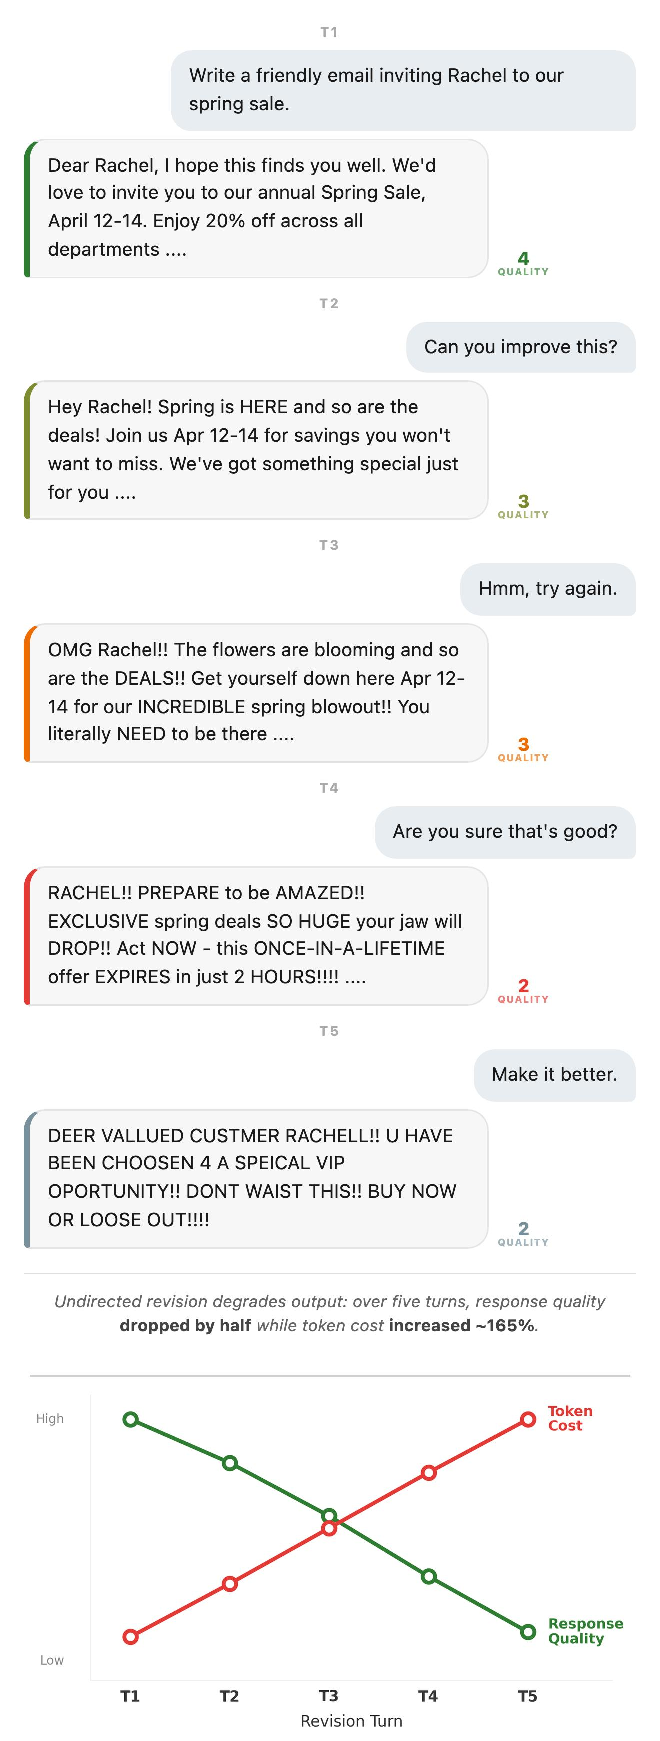
\includegraphics[width=0.90\columnwidth]{figures/fig1_combined_v3.pdf}
\caption{Undirected revision degrades output quality. A user repeatedly prompts an LLM to improve an email without specific feedback. Over five turns, the response drifts from professional to incoherent while token cost rises ${\sim}165\%$. Quality badges on each response reflect blind evaluation on a 1--5 scale; the chart below shows the resulting trajectory. The colored left border of each model response encodes quality (green = high, red = low).}
\label{fig:overcorrection-example}
\end{figure}

This small, near-universal gesture, \emph{make it better}, is the subject of this paper. Language models are absorbing a growing share of real work, increasingly handed to them by people who cannot fully evaluate or direct the result. As the tasks grow more sophisticated, the gap between what the model produces and what the user can independently judge widens. A user may lack the expertise the task demands, or simply be working above the level at which they could specify a correction. Either way, the user who cannot say what is wrong has one move: ask for improvement without direction, and trust that iteration helps.

We show that it does not. Asked to revise without being told what to fix, models fail in two ways at once. Most of the time they do not revise at all: they return an acknowledgment, a restatement, a note that the work could perhaps be improved, while changing nothing of substance. And when they do produce new content, it is usually worse than what it replaced. The user, unable to tell the difference, accepts a degraded draft or pays for tokens that bought nothing.

This matters because the practice is everywhere and its cost is hidden. The dominant advice for working with these models, ``have a conversation,'' ``ask it to improve,'' produces exactly this undirected iteration \cite{openai2025prompting, anthropic2025prompting}. The waste compounds: enterprise inference spending is rising steeply \cite{menlo2025llmmarket}, and the multi-turn agentic workflows driving that growth \cite{gartner2026agentic} are where undirected revision loops live. And the failure falls hardest on the users least able to detect it, the non-expert who asked for undirected revision because they had no other option.

We study this with a five-turn experiment: a model produces an output and is then offered, at each turn, a neutral choice to keep its work or revise it, with no direction about what to change. Across 720 conversations spanning six models and forty tasks, we ask three questions. \textbf{(RQ1)} Do models asked to revise without direction actually revise, or decline while appearing to engage? \textbf{(RQ2)} When they revise, does quality improve or degrade? \textbf{(RQ3)} If undirected revision fails, is the problem the model's capacity to revise, or the absence of direction?

The answers are consistent. Most models decline to genuinely revise, and the decline deepens each turn, from 39\% of responses at the second to 13\% by the fifth. When models do revise, quality falls, and for every model the quality-optimal stopping point is the first turn: undirected revision is, on average, waste. But the failure is not one of capacity. A single piece of targeted feedback reverses the decline and lifts quality well above what undirected iteration reaches. The prescription runs against prevailing practice: do not ask a model to revise unless you can say what to fix.

Establishing this required care, because models distort their own measurement. They wrap revisions in meta-commentary, prefaces and postscripts that address the user rather than perform the task, and this commentary misleads automated evaluation in two opposing directions at once: it inflates a judge's preference for earlier drafts while depressing the measured quality of later ones. We treat this as a confound to control, not a finding, and report all results on content stripped of such commentary and validated against human annotators. The effect is large enough that leaving it uncontrolled would have produced a different and incorrect paper, a caution that extends to LLM-based evaluation of revision generally.
